% Example from below
% https://www.overleaf.com/learn/latex/Learn_LaTeX_in_30_minutes
\documentclass[12pt, A4]{article} %  defines the overall class (type) of document.
%if we use book class instead of article, we can use \chapter{Let's begin} before  \section{•}
\usepackage{graphicx} %LaTeX package to import graphics
%\usepackage[bottom=0.5cm, right=1.5cm, left=1.5cm, top=1.5cm]{geometry} % to change the margin of Page
\graphicspath{{images/}} %configuring the graphicx package


% ///////Below is components for title page ///////////
\title{A Beginner's Guide to DGUS V7.641}
\author{Sannan Ahmed}
\date{\today} %\date{August 2022}
%/////////////////////////////


% any thing above \begin is called preamble

\begin{document}

%if you press two "enter" key then new paragraph will created

% ///////this is to make a title page///////////
\begin{titlepage}
\maketitle
\thispagestyle{empty} %this will clear the number from the title page
\end{titlepage}
%////////////////////////////////

%to add a table of contents (table of contents need to be updated (cut then Quick Build & paste then Quick Build) if any content changes.

\tableofcontents
%to add new line
\newpage

\section{Gray word font}

It is created using software Gray word library generator from DWIN. It has greater experience than 0 word font. For gray word font we have to use 8bit encapsulation.

% The \includegraphcs command is provided (implemented) by the graphicx package
\begin{figure}[!htb] %[!htb] is used to place image where it is in editor
	\centering
	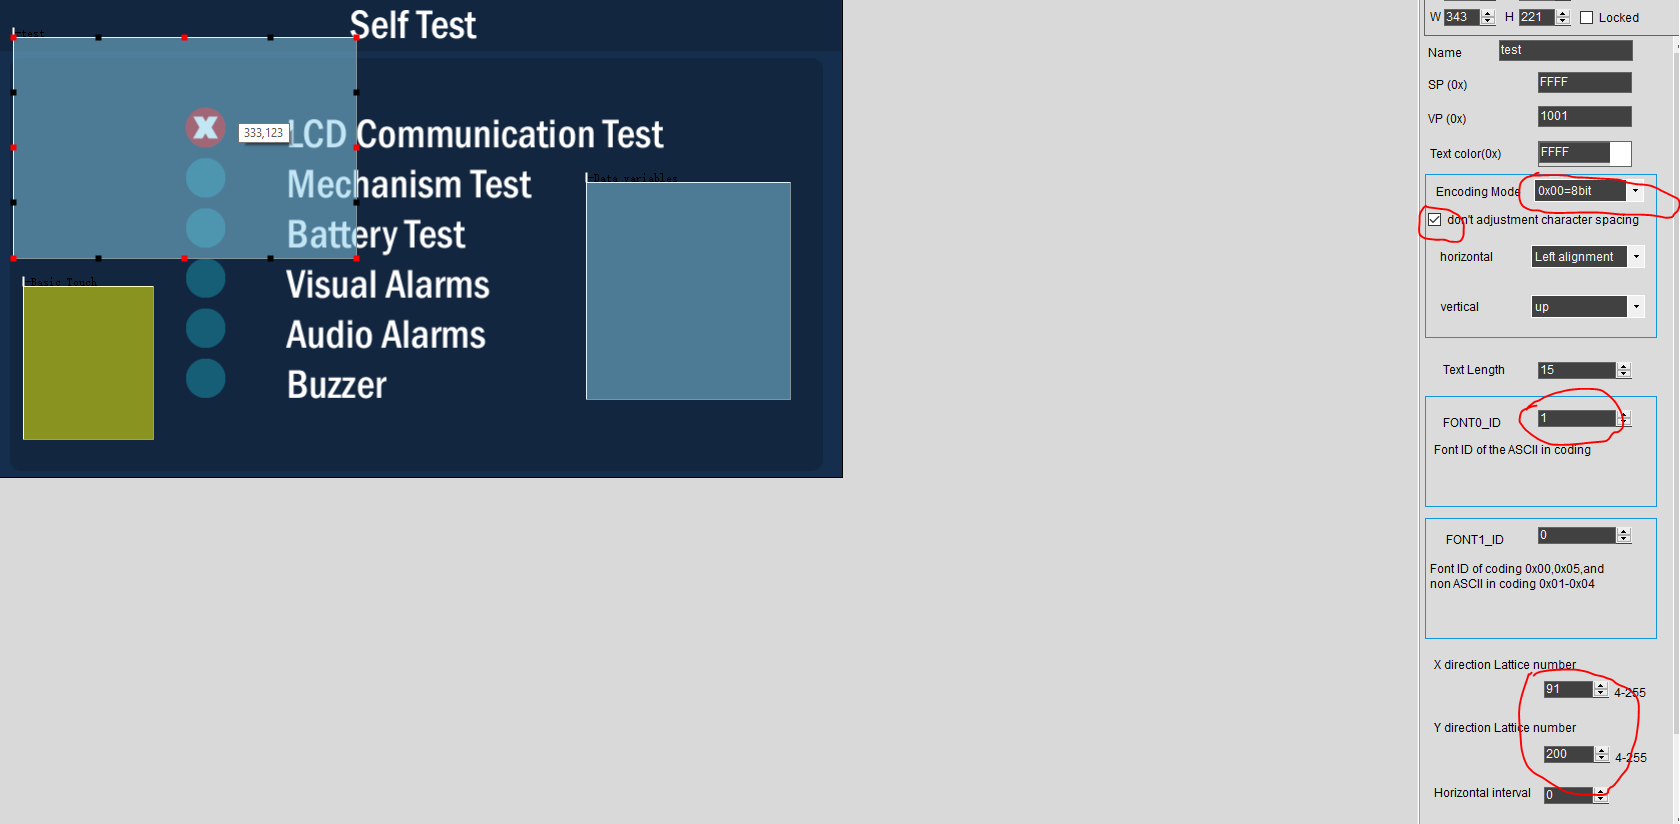
\includegraphics[width=14cm]{grayFont} 
	\caption{This picture shows necessary setting.}
\end{figure}

\begin{figure}[!htb] %[!htb] is used to place image where it is in editor
	\centering
	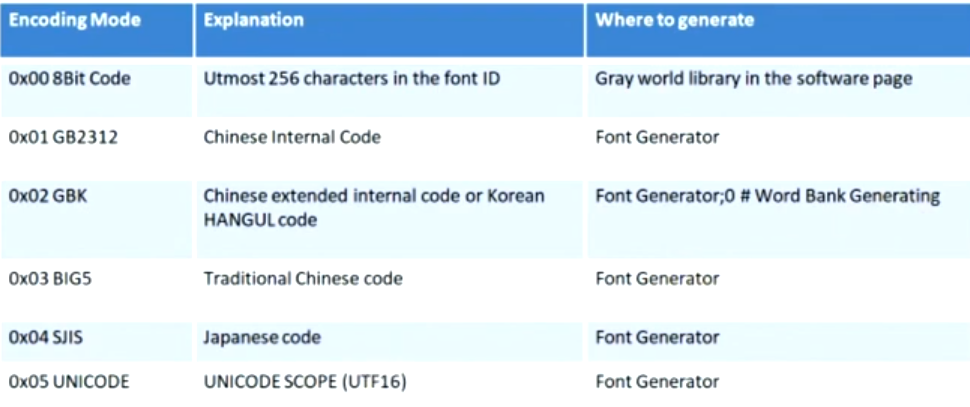
\includegraphics[width=14cm]{encoding} 
	\caption{This picture encoding settings.}
\end{figure}



%this is how to go on new page
\newpage


\section{data send serially}

\emph{Note: First of all enable Touch variable automatic upload 1=On from system configuration. This is needed to send data from Syncrodata return and return key code functions of DGUS software}

\begin{figure}[!htb] %[!htb] is used to place image where it is in editor
	\centering
	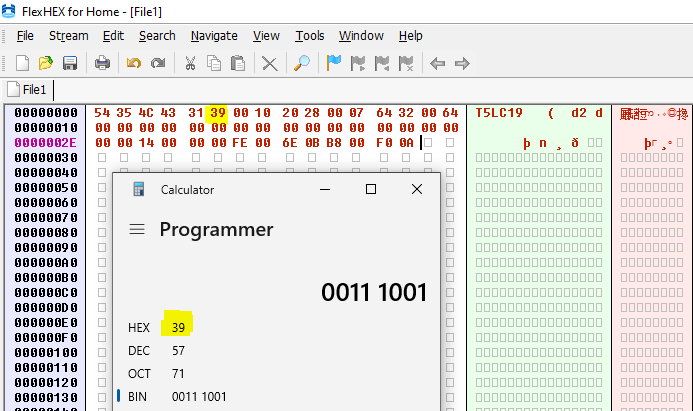
\includegraphics[width=10cm]{autoupload} 
	\caption{auto Upload commmand}
\end{figure}

following image shows the command through which data can be send/receive from MCU. 
\\ Following command will change the page. (it will make use of system variable)


\begin{figure}[!htb] %[!htb] is used to place image where it is in editor
	\centering
	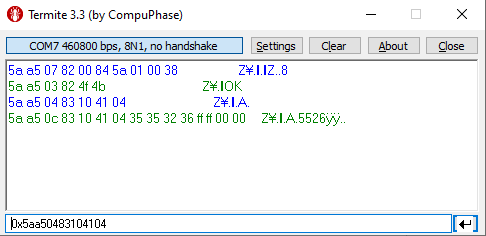
\includegraphics[width=10cm]{receive} 
	\caption{send/receive from MCU command (Data received is : 5523)}
\end{figure}

\newpage


\section{page change from synchrodata return}

Page can be changed from synchodata return. see the below image.

\begin{figure}[!htb] %[!htb] is used to place image where it is in editor
	\centering
	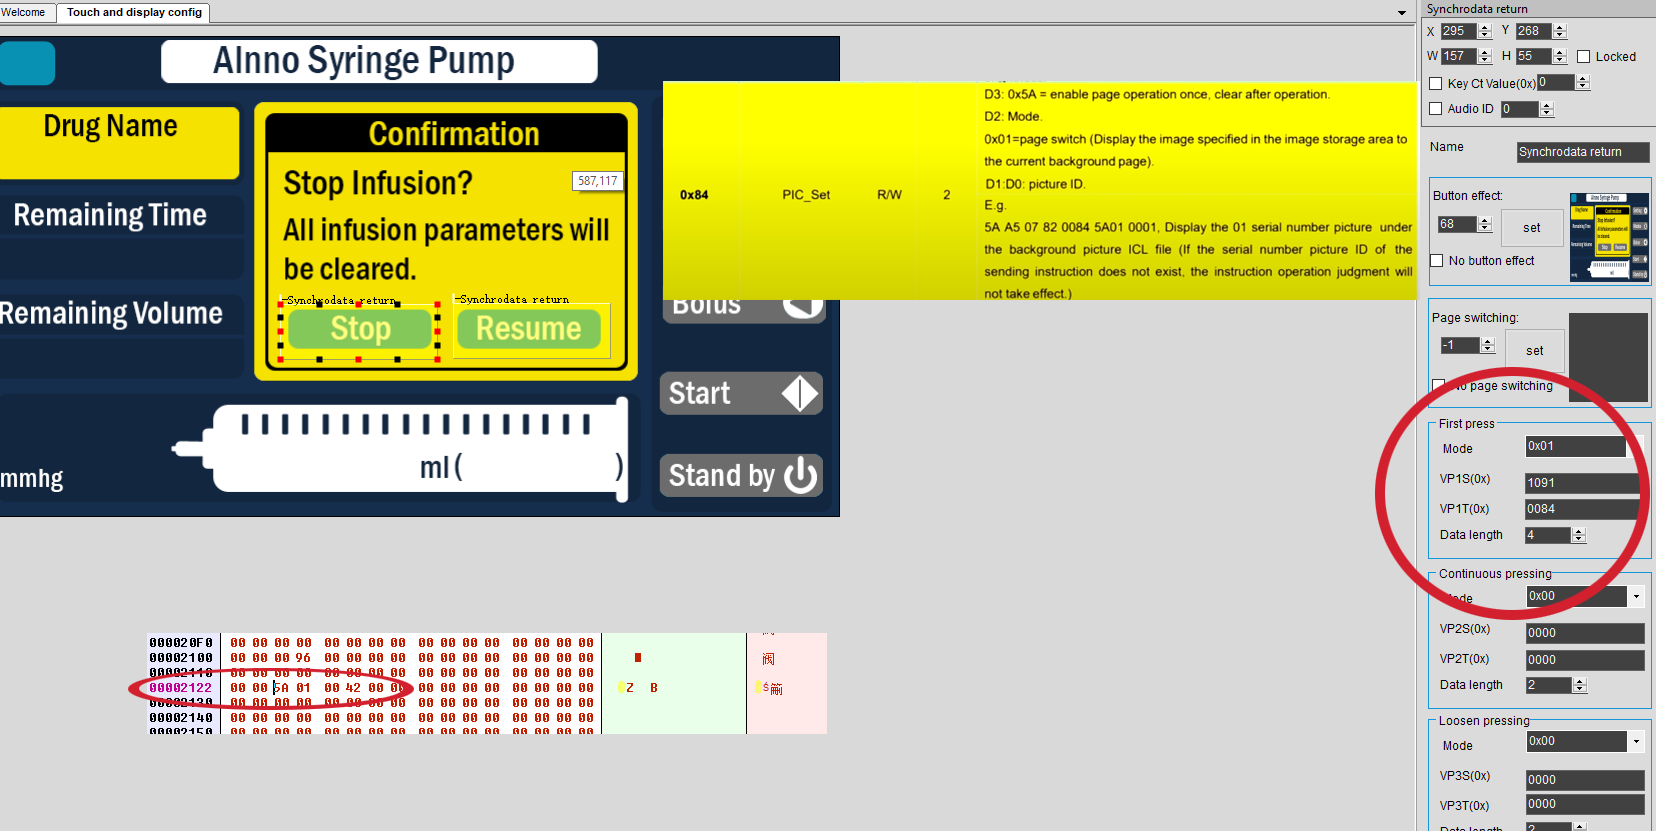
\includegraphics[width=14cm]{pageChageCommand} 
	\caption{pageChageCommand}
\end{figure}

\newpage

\section{Save variable in Nor Flash}

Address of nor flash, it must be an even number, the range is 0x000000 - 0x027FFE, and then one address corresponds to 2 bytes, that is the total capacity is 320KB.\\

\emph{for NOR flash database site \\
Each ID corresponds to 2KWords memory with ID range of 0 - 79.
The database is located in on-chip NOR FLASH of 160KWords (320 KB). It
can be used to save user data or DWIN OS program library files.}


\begin{figure}[!htb] %[!htb] is used to place image where it is in editor
	\centering
	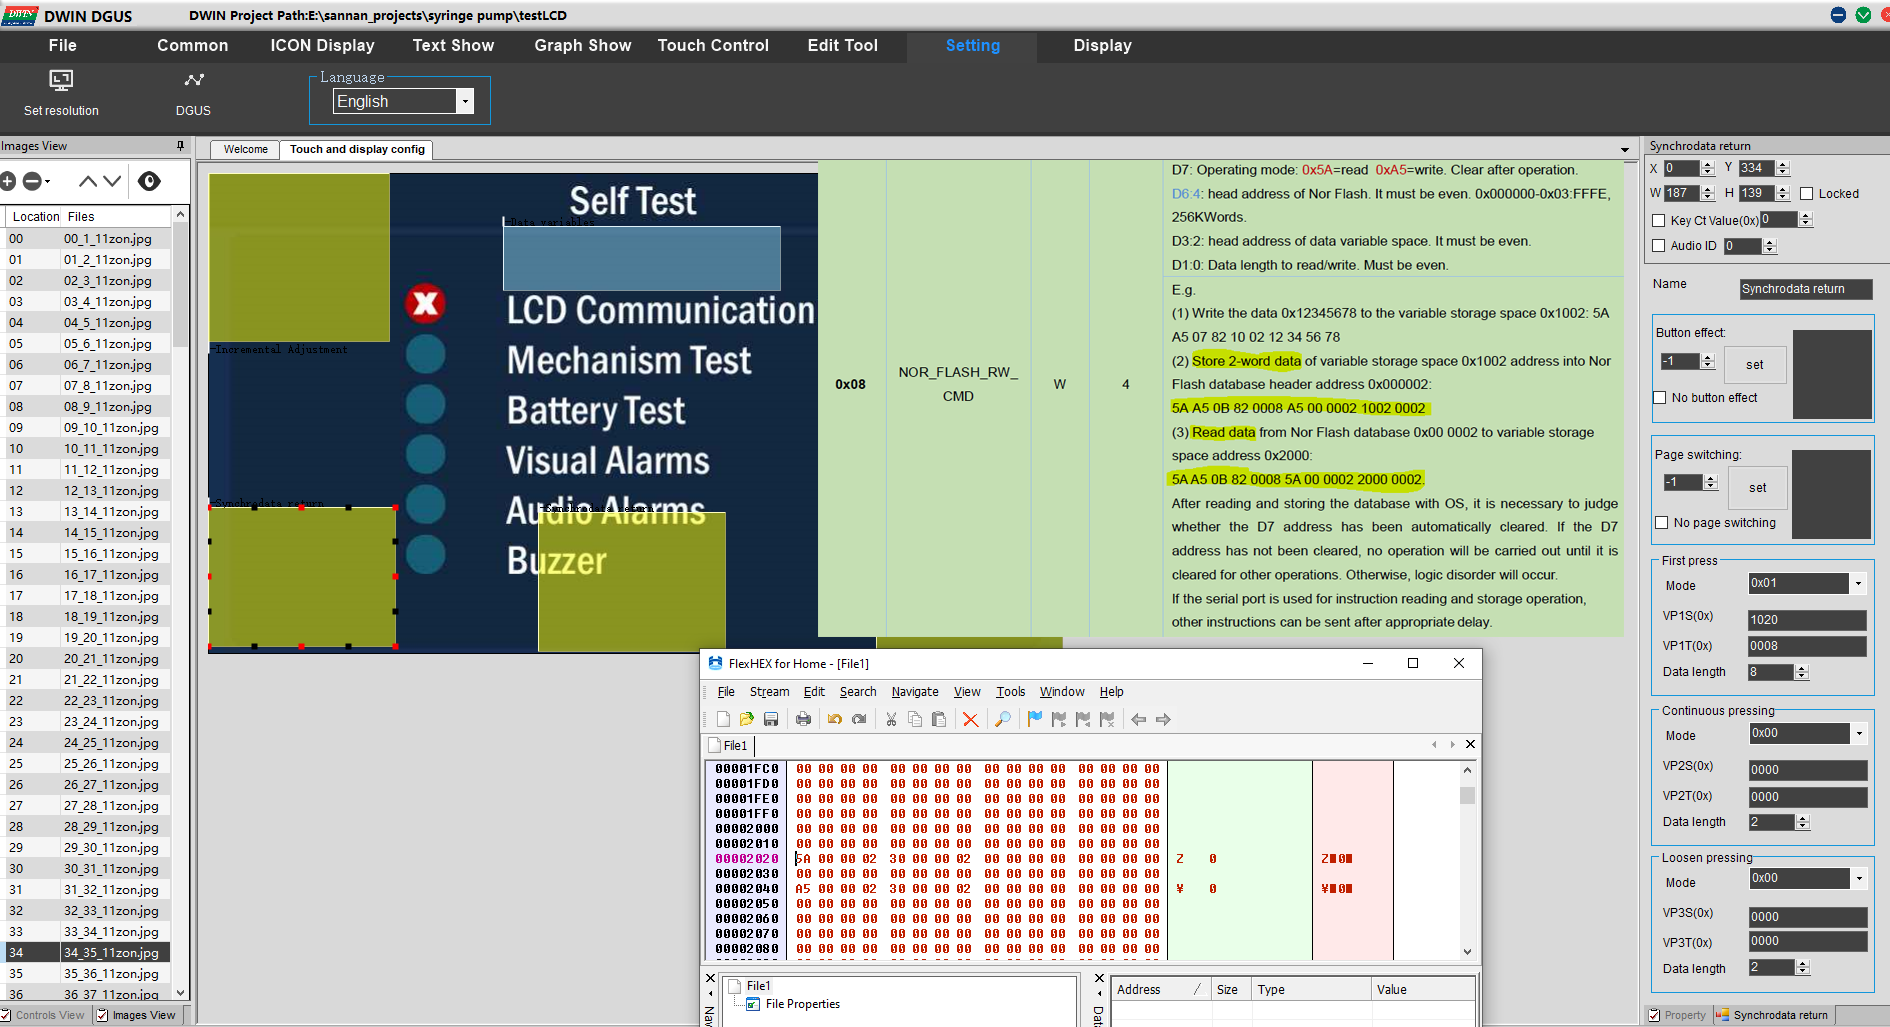
\includegraphics[width=14cm]{NorFlash} 
	\caption{NorFlash}
\end{figure}

\newpage

\end{document}